\documentclass[11pt,aspectratio=169]{beamer}

\usepackage{amsmath,amssymb,bm}
\usepackage{graphicx}

\usetheme{default}
\setbeamertemplate{navigation symbols}{}
\setbeamertemplate{headline}{}
\setbeamertemplate{footline}{}
\setbeamertemplate{frametitle}{%
  \vspace{0.25cm}%
  \insertframetitle\par
  \vspace{0.08cm}%
  \hrule
}
\setbeamercolor{normal text}{fg=black,bg=white}
\setbeamercolor{frametitle}{fg=black,bg=white}
\setbeamercolor{structure}{fg=black}
\setbeamersize{text margin left=0.7cm,text margin right=0.7cm}

\newcommand{\dd}{\,\mathrm{d}}
\newcommand{\Om}{\Omega}
\newcommand{\Gam}{\Gamma}
\newcommand{\Th}{\mathcal T_h}
\newcommand{\Vzero}{\mathcal V_0}
\newcommand{\Vhzero}{\mathcal V_{h,0}}
\newcommand{\norm}[2][]{\left\lVert#2\right\rVert_{#1}}
\newcommand{\seminorm}[2][]{\left\lvert#2\right\rvert_{#1}}
\newcommand{\bx}{\bm x}
\newcommand{\bu}{\bm u}
\newcommand{\bv}{\bm v}
\newcommand{\bK}{\bm K}
\newcommand{\bV}{\bm V}
\newcommand{\bI}{\bm I}

\graphicspath{{figures/}}

\begin{document}

\begin{frame}[plain]
  \centering
  \vfill
  {\LARGE\bfseries A Priori Error Analysis\par}
  \vspace{0.45cm}
  {\large Galerkin orthogonality, best approximation, and interpolation\par}
  \vfill
\end{frame}

\section{Problem setting and error measures}

\begin{frame}{Lecture outline}
The finite element computation gives $u_h$. We now ask how $u_h$ compares
with the exact weak solution $u$.

\begin{enumerate}
  \item State the continuous and discrete variational problems.
  \item Introduce the $L^2$, $H^1$, and energy measures of error.
  \item Derive Galerkin orthogonality and its best-approximation consequence.
  \item Prove C\'ea's lemma.
  \item Construct the nodal interpolant and obtain the one-dimensional
  interpolation estimates.
\end{enumerate}

\vspace{0.2cm}
The lecture ends with linear interpolation in one dimension, Section 7.5.2.
\end{frame}

\begin{frame}{Continuous and discrete problems}
Let
\[
  \Vzero=H^1_{0,\Gam_D}(\Om),
  \qquad
  a(w,v)=\int_\Om k\,\nabla w\cdot\nabla v\,\dd\bx .
\]
The continuous problem is
\[
  \boxed{
  \text{find }u\in\Vzero:\quad
  a(u,v)=\ell(v)
  \quad\forall v\in\Vzero.}
\]

For a conforming finite element space $\Vhzero\subset\Vzero$, the discrete
problem is
\[
  \boxed{
  \text{find }u_h\in\Vhzero:\quad
  a(u_h,v_h)=\ell(v_h)
  \quad\forall v_h\in\Vhzero.}
\]

The two problems use the same bilinear and linear forms. Only the spaces differ.
\end{frame}

\begin{frame}{Assumptions for the analysis}
We assume throughout this lecture that
\begin{itemize}
  \item $\Om$ is a bounded Lipschitz domain and $\Gam_D$ has positive
  boundary measure;
  \item $0<k_0\leq k(\bx)\leq k_1$ almost everywhere in $\Om$;
  \item $\Th$ is conforming and resolves the boundary partition;
  \item $\Vhzero$ is a continuous Lagrange space of degree $p\geq1$ with
  homogeneous values on $\Gam_D$; and
  \item the forms $a$ and $\ell$ are evaluated exactly.
\end{itemize}

\vspace{0.2cm}
Approximating the forms by quadrature or approximating boundary data adds a
consistency error. Such modifications are called \textbf{variational crimes}.
They are outside today's analysis.
\end{frame}

\begin{frame}{Continuity and coercivity}
The analysis uses two estimates:
\[
  |a(w,v)|
  \leq M\norm[H^1(\Om)]{w}\norm[H^1(\Om)]{v},
  \qquad w,v\in\Vzero,
\]
and
\[
  a(v,v)
  \geq\alpha\norm[H^1(\Om)]{v}^2,
  \qquad v\in\Vzero.
\]

For scalar diffusion,
\[
  M=k_1,
  \qquad
  \alpha=\frac{k_0}{1+C_P^2},
  \qquad
  \frac{M}{\alpha}=\frac{k_1}{k_0}(1+C_P^2).
\]

The constants depend on the coefficient and the domain, but not on the mesh
size $h$ or polynomial degree $p$.
\end{frame}

\begin{frame}{Existence and stability of the discrete solution}
Because $\Vhzero$ is a finite-dimensional subspace of $\Vzero$, the same
continuity and coercivity estimates hold on $\Vhzero$.

The Lax--Milgram theorem therefore gives a unique finite element solution and
\[
  \norm[H^1(\Om)]{u_h}
  \leq
  \frac{1}{\alpha}\norm[\Vzero^*]{\ell}.
\]

The same fact appears in the algebraic system. For any nonzero coefficient
vector $\bV$ representing $v_h\in\Vhzero$,
\[
  \bV^T\bK_{ff}\bV
  =a(v_h,v_h)
  \geq\alpha\norm[H^1(\Om)]{v_h}^2>0.
\]
When $a$ is symmetric, the reduced stiffness matrix $\bK_{ff}$ is symmetric
positive definite.
\end{frame}

\begin{frame}{Measures of the error}
Define
\[
  e=u-u_h.
\]
Because $u,u_h\in\Vzero$, the error also belongs to $\Vzero$.

\begin{align*}
  \norm[L^2(\Om)]{e}
  &\quad\text{measures error in the solution values},\\[2mm]
  \seminorm[H^1(\Om)]{e}
  =\norm[L^2(\Om;\mathbb R^d)]{\nabla e}
  &\quad\text{measures error in the gradient},\\[2mm]
  \norm[H^1(\Om)]{e}
  =\bigl(\norm[L^2(\Om)]{e}^2
  +\seminorm[H^1(\Om)]{e}^2\bigr)^{1/2}
  &\quad\text{measures both}.
\end{align*}

For diffusion, the gradient error determines the flux error. For elasticity,
it determines the strain error.
\end{frame}

\begin{frame}{Energy norm}
Suppose $a$ is symmetric, continuous, and coercive on $\Vzero$. Define
\[
  \boxed{\norm[a]{v}=a(v,v)^{1/2}.}
\]
This is a norm because $a$ is an inner product on $\Vzero$.

For scalar diffusion,
\[
  \norm[a]{v}^2
  =\int_\Om k\,|\nabla v|^2\,\dd\bx.
\]
The coefficient bounds give
\[
  \sqrt{k_0}\,\seminorm[H^1(\Om)]{v}
  \leq\norm[a]{v}
  \leq\sqrt{k_1}\,\seminorm[H^1(\Om)]{v}.
\]

The energy norm weights the gradient by the material coefficient $k$.
\end{frame}

\begin{frame}{Energy norm and the $H^1$ norm}
On $\Vzero$, the Poincar\'e inequality gives
\[
  \norm[H^1(\Om)]{v}^2
  \leq(1+C_P^2)\seminorm[H^1(\Om)]{v}^2.
\]
Combining this with the coefficient bounds gives
\[
  \boxed{
  \sqrt{\frac{k_0}{1+C_P^2}}\,
  \norm[H^1(\Om)]{v}
  \leq
  \norm[a]{v}
  \leq
  \sqrt{k_1}\,\norm[H^1(\Om)]{v}.}
\]

Thus convergence in the energy norm is equivalent to convergence in the
$H^1$ norm on $\Vzero$. The numerical values of the two norms need not be
equal.
\end{frame}

\begin{frame}{Energy norm for an axial bar}
For an axial bar with $v(0)=0$,
\[
  a(w,v)=\int_0^L AE\,w'v'\,\dd x,
  \qquad
  \norm[a]{e}^2=\int_0^L AE\,(e')^2\,\dd x.
\]

The energy norm weights the strain error by the axial rigidity. When $AE=1$,
\[
  \norm[a]{e}=\seminorm[H^1(0,L)]{e}.
\]
Because $e(0)=0$, the Poincar\'e inequality makes this seminorm equivalent to
the full $H^1(0,L)$ norm.

\vspace{0.2cm}
Without an essential boundary condition, a nonzero constant displacement has
zero strain and zero value of $a(v,v)$. The energy expression is then only a
seminorm until rigid translations are removed.
\end{frame}

\section{Galerkin orthogonality and best approximation}

\begin{frame}{Galerkin orthogonality}
Every $v_h\in\Vhzero$ is also an admissible test function in the continuous
problem. Hence
\[
  a(u,v_h)=\ell(v_h),
  \qquad
  a(u_h,v_h)=\ell(v_h).
\]
Subtracting the discrete equation from the continuous equation gives
\[
  \boxed{
  a(u-u_h,v_h)=0
  \qquad\forall v_h\in\Vhzero.}
\]

For symmetric $a$, this says that the error $u-u_h$ is orthogonal to the
discrete space in the energy inner product.
\end{frame}

\begin{frame}{Conditions behind the orthogonality relation}
The derivation uses two facts.

\begin{enumerate}
  \item \textbf{Conformity:} $\Vhzero\subset\Vzero$. Every discrete test
  function can be inserted into the continuous problem.
  \item \textbf{The same forms:} the continuous and discrete problems use
  the same $a$ and $\ell$.
\end{enumerate}

Define the residual associated with $u_h$ by
\[
  R(v)=\ell(v)-a(u_h,v),
  \qquad v\in\Vzero.
\]
Galerkin orthogonality is equivalent to
\[
  R(v_h)=0\qquad\forall v_h\in\Vhzero.
\]
The residual generally does not vanish on test functions outside the discrete
space.
\end{frame}

\begin{frame}{Pythagorean identity in the energy norm}
For any $v_h\in\Vhzero$,
\[
  u-v_h=(u-u_h)+(u_h-v_h).
\]
The second term belongs to $\Vhzero$, so Galerkin orthogonality gives
\[
  a(u-u_h,u_h-v_h)=0.
\]
For symmetric $a$,
\[
  \boxed{
  \norm[a]{u-v_h}^2
  =\norm[a]{u-u_h}^2+\norm[a]{u_h-v_h}^2.}
\]

The same conclusion follows from the quadratic energy functional:
\[
  \Pi(v_h)-\Pi(u)=\frac12\norm[a]{u-v_h}^2.
\]
Thus the Galerkin solution is also the Ritz minimizer over $\Vhzero$.
\end{frame}

\begin{frame}{Best approximation from a discrete space}
\begin{columns}[T,onlytextwidth]
  \begin{column}{0.42\textwidth}
    For a finite-dimensional subspace $V_h\subset V$, define
    \[
      E_V(u;V_h)=\min_{v_h\in V_h}\norm[V]{u-v_h}.
    \]
    This is the smallest distance from $u$ to a point in $V_h$. The minimizing
    function depends on the selected norm.

    \vspace{0.25cm}
    For the energy inner product, Galerkin orthogonality identifies $u_h$ as
    the orthogonal projection of $u$ onto $V_h$.
  \end{column}
  \begin{column}{0.55\textwidth}
    \centering
    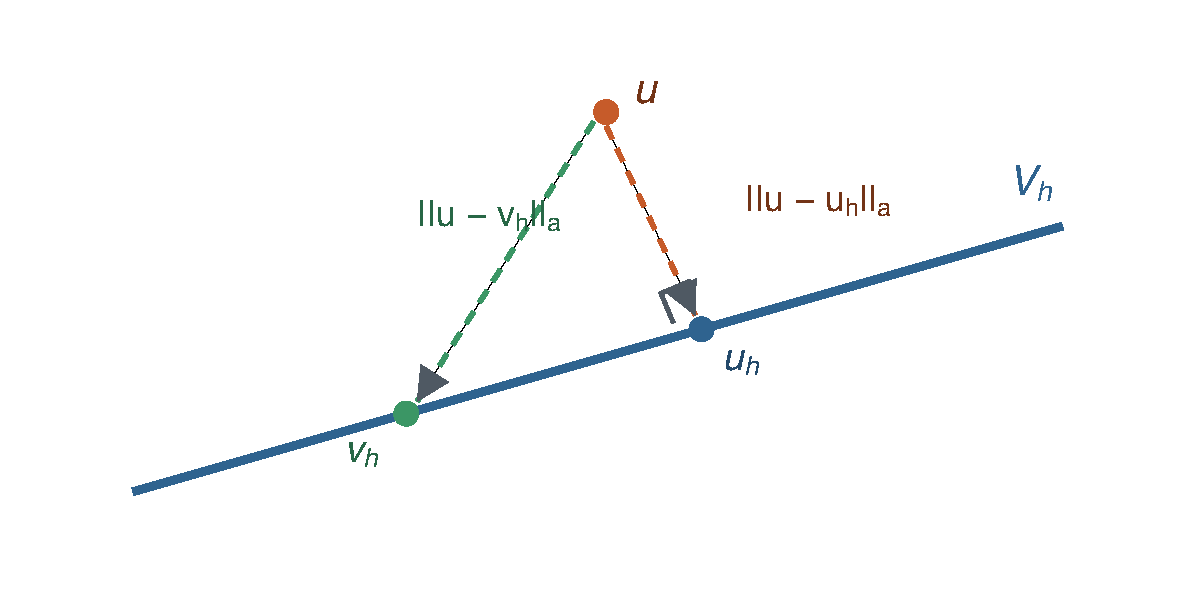
\includegraphics[width=0.98\textwidth]{c7_best_approximation.pdf}
  \end{column}
\end{columns}
\end{frame}

\begin{frame}{A weighted best-approximation example}
Let
\[
  V=\mathbb R^2,
  \qquad
  V_h=\operatorname{span}\{(1,1)\},
  \qquad
  \bu=(1,0),
\]
and define
\[
  a(\bx,\bv)=4x_1v_1+x_2v_2,
  \qquad
  \norm[a]{\bx}=\sqrt{4x_1^2+x_2^2}.
\]
Every vector in $V_h$ has the form $\bv_h=t(1,1)$. Therefore
\[
  \norm[a]{\bu-\bv_h}^2=4(1-t)^2+t^2.
\]
Minimizing this quadratic gives
\[
  t=\frac45,
  \qquad
  \bu_h=\left(\frac45,\frac45\right).
\]
The Euclidean closest point is $\tfrac12(1,1)$. The discrete space is the
same, but the norm changes the best approximation.
\end{frame}

\section{C\'ea's lemma}

\begin{frame}{C\'ea's lemma}
Let $V$ be a Hilbert space and $V_h\subset V$ a finite-dimensional subspace.
Assume that
\[
  |a(w,v)|\leq M\norm[V]{w}\norm[V]{v},
  \qquad
  a(v,v)\geq\alpha\norm[V]{v}^2.
\]
If $u$ and $u_h$ solve the continuous and discrete Galerkin problems, then
\[
  \boxed{
  \norm[V]{u-u_h}
  \leq
  \frac{M}{\alpha}
  \inf_{v_h\in V_h}\norm[V]{u-v_h}.}
\]

The estimate compares the computed error with the smallest error attainable
in $V_h$.
\end{frame}

\begin{frame}{Proof of C\'ea's lemma: coercivity and orthogonality}
Let $e=u-u_h$ and choose any $v_h\in V_h$. Coercivity gives
\[
  \alpha\norm[V]{e}^2\leq a(e,e).
\]
Insert
\[
  e=(u-v_h)+(v_h-u_h)
\]
in the second argument:
\[
  a(e,e)
  =a(e,u-v_h)+a(e,v_h-u_h).
\]
Because $v_h-u_h\in V_h$, Galerkin orthogonality gives
\[
  a(e,v_h-u_h)=0.
\]
Hence
\[
  \alpha\norm[V]{e}^2\leq a(e,u-v_h).
\]
\end{frame}

\begin{frame}{Proof of C\'ea's lemma: continuity}
Continuity of $a$ gives
\[
  \alpha\norm[V]{e}^2
  \leq
  M\norm[V]{e}\norm[V]{u-v_h}.
\]
If $e\ne0$, divide by $\alpha\norm[V]{e}$:
\[
  \norm[V]{u-u_h}
  \leq
  \frac{M}{\alpha}\norm[V]{u-v_h}.
\]
This holds for every $v_h\in V_h$. Taking the infimum gives C\'ea's estimate.

\vspace{0.25cm}
For diffusion in the $H^1$ norm,
\[
  \frac{M}{\alpha}
  =\frac{k_1}{k_0}(1+C_P^2).
\]
This factor does not depend on $h$ or $p$.
\end{frame}

\begin{frame}{Best approximation in the energy norm}
When $a$ is symmetric, the Pythagorean identity gives
\[
  \norm[a]{u-v_h}^2
  =\norm[a]{u-u_h}^2+\norm[a]{u_h-v_h}^2.
\]
The final term is nonnegative, so
\[
  \boxed{
  \norm[a]{u-u_h}
  =\min_{v_h\in V_h}\norm[a]{u-v_h}.}
\]

Thus the constant in the energy norm is exactly one. To estimate the finite
element error, it now suffices to choose one convenient $v_h\in V_h$ and
estimate $\norm[a]{u-v_h}$. The nodal interpolant provides that choice.
\end{frame}

\section{Finite element interpolation}

\begin{frame}{Finite element interpolant}
Let $V_h$ be a Lagrange finite element space with global nodes $\bx_i$ and
nodal basis functions $\phi_i$. For a continuous function $u$, define
\[
  \boxed{
  \mathcal I_hu
  =\sum_{i=1}^{N_n}u(\bx_i)\phi_i.}
\]
The interpolant belongs to $V_h$ and satisfies
\[
  \mathcal I_hu(\bx_i)=u(\bx_i)
  \qquad i=1,\ldots,N_n.
\]

On an element $\mathcal K_e$,
\[
  (\mathcal I_hu)|_{\mathcal K_e}
  =\mathcal I_e(u|_{\mathcal K_e}).
\]
Thus the global interpolant can be constructed cell by cell from the nodal
values of $u$.
\end{frame}

\begin{frame}{Interpolation on a triangular mesh}
  \centering
  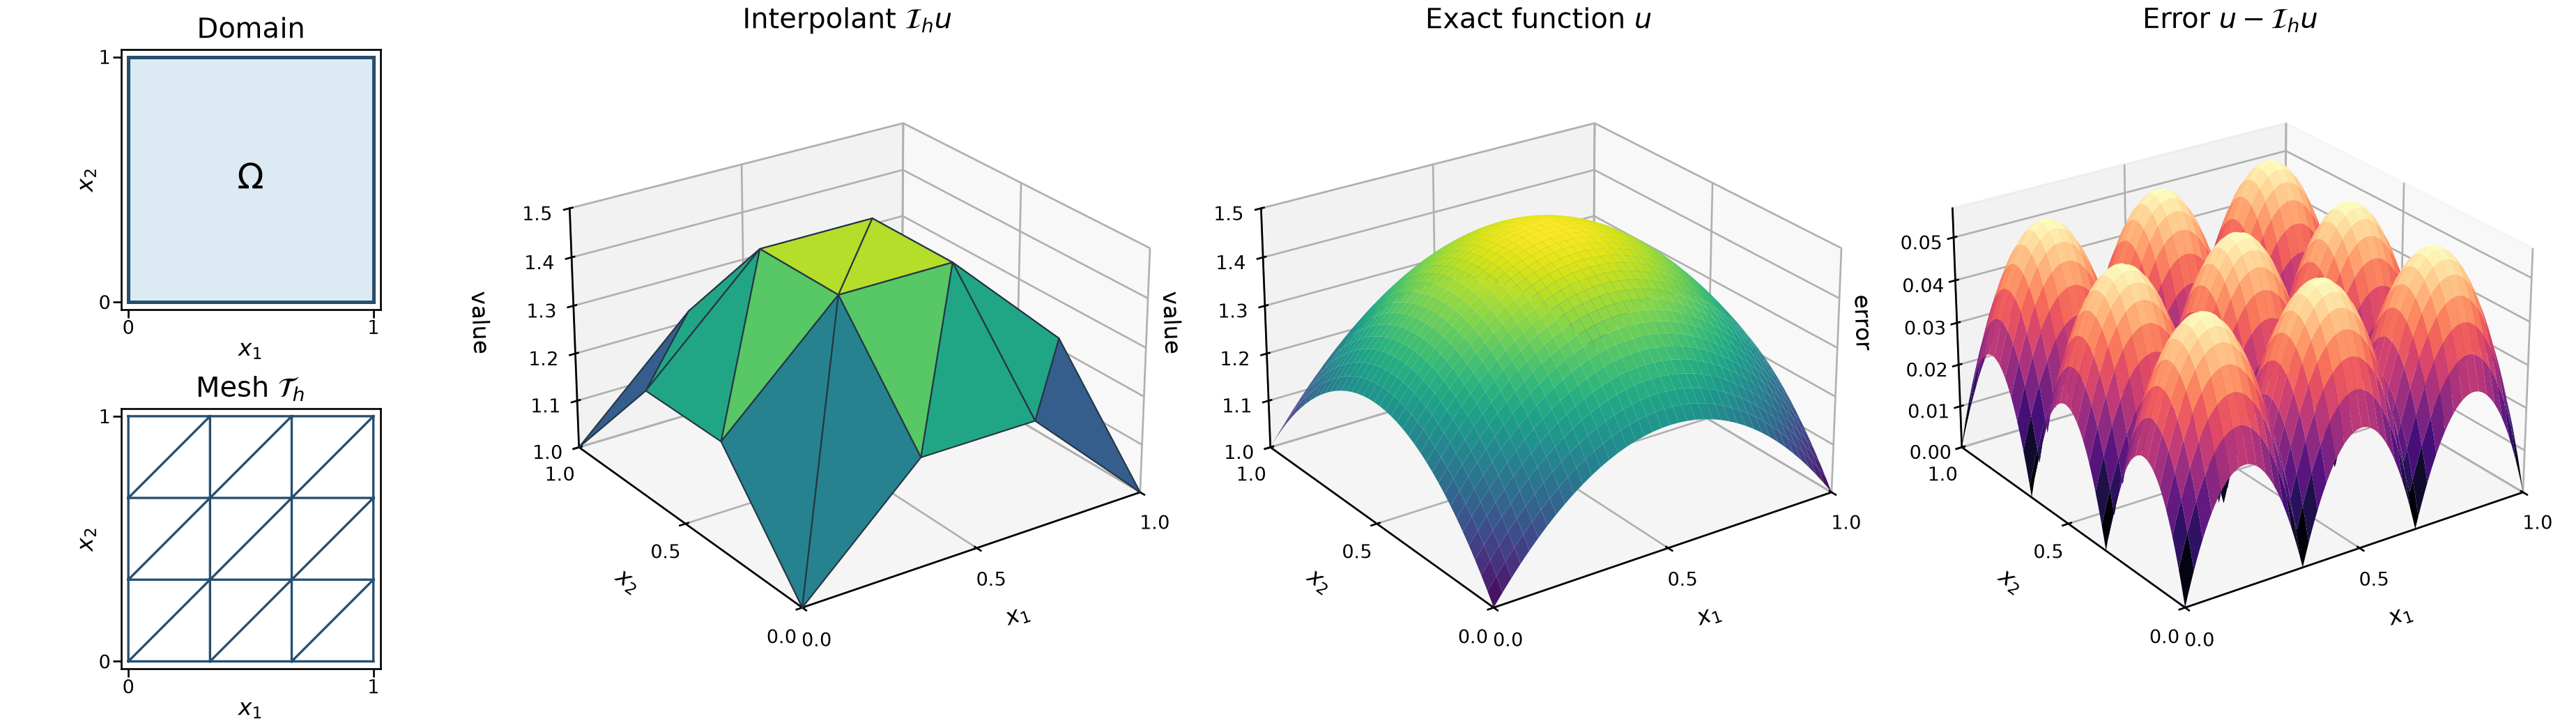
\includegraphics[width=0.99\textwidth]{c7_interpolation_2d.png}

  \vspace{0.05cm}
  The coarse mesh defines the $P_1$ interpolant. The finer plotting points
  only display the exact function and the error smoothly; they are not
  additional finite element nodes. For this quadratic and uniform mesh, the
  error pattern repeats on every triangle up to translation or reflection.
\end{frame}

\begin{frame}{Interpolation after uniform refinement}
  \centering
  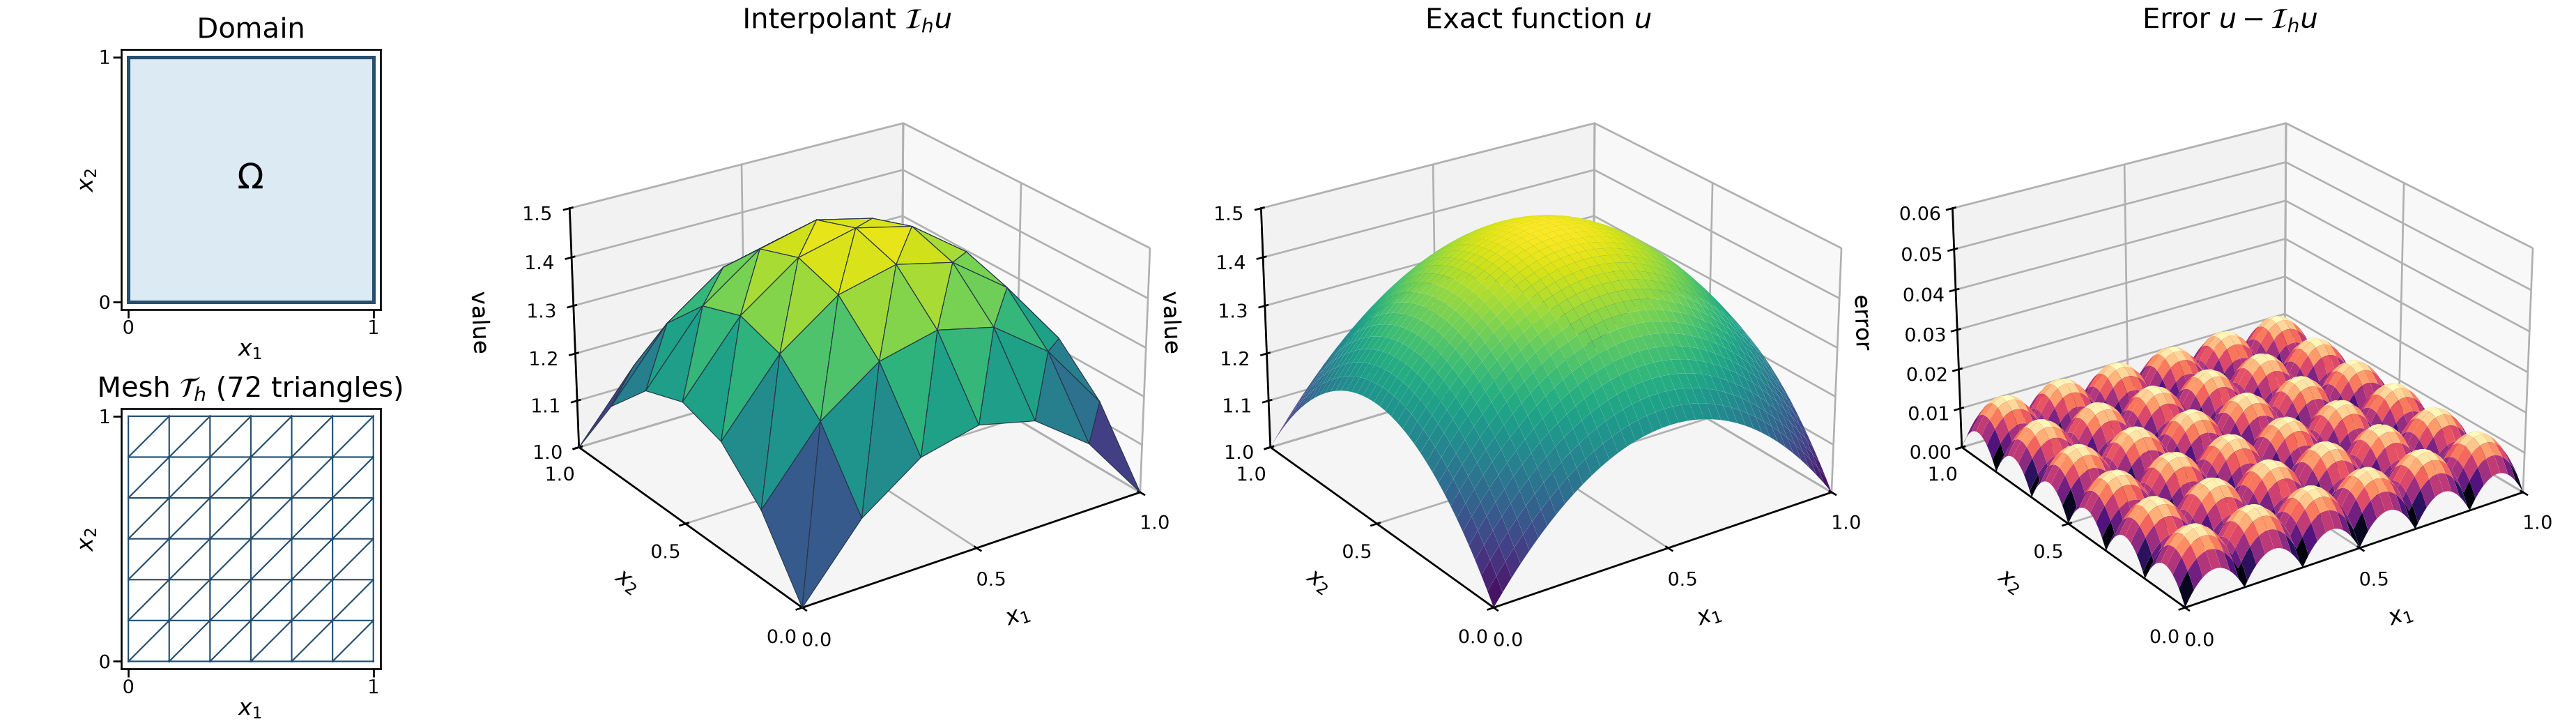
\includegraphics[width=0.99\textwidth]{c7_interpolation_2d_fine.png}

  \vspace{0.05cm}
  Halving the grid spacing increases the mesh from 18 to 72 triangles. With
  the same vertical scales in both figures, the maximum error decreases from
  $1/18$ to $1/72$, a factor of four.
\end{frame}

\begin{frame}{Properties and regularity of the interpolant}
Three properties will be used in the error estimates.
\begin{enumerate}
  \item \textbf{Locality:} $(\mathcal I_hu)|_{\mathcal K_e}$ depends only on
  the degrees of freedom of $\mathcal K_e$.
  \item \textbf{Polynomial reproduction:} if
  $u|_{\mathcal K_e}$ belongs to the local finite element space, then
  $\mathcal I_eu=u$ on $\mathcal K_e$.
  \item \textbf{Boundary values:} if $u=0$ on $\Gam_D$ and the mesh resolves
  $\Gam_D$, then $\mathcal I_hu\in\Vhzero$.
\end{enumerate}

\vspace{0.2cm}
The nodal interpolant requires point values. In one dimension, $H^1$
functions are continuous. In two and three dimensions, a general $H^1$
function need not be continuous, so the estimates will assume additional
regularity, commonly $u\in H^2(\Om)$.
\end{frame}

\section{Linear interpolation in one dimension}

\begin{frame}{A four-element linear mesh}
Consider $u(x)=1+x(1-x)$ on $[0,1]$. Use four uniform linear elements with
five nodes:
\[
  x_1=0,
  \qquad x_2=\frac14,
  \qquad x_3=\frac12,
  \qquad x_4=\frac34,
  \qquad x_5=1.
\]

On $\mathcal K_e=[x_e,x_{e+1}]$,
\[
  \mathcal I_eu
  =u(x_e)\phi_1^e+u(x_{e+1})\phi_2^e.
\]

The interpolant agrees with $u$ at both element nodes and is linear between
them. Adjacent local interpolants share the same value at their common node,
so the global interpolant is continuous.
\end{frame}

\begin{frame}{Exact function, interpolant, and error}
  \centering
  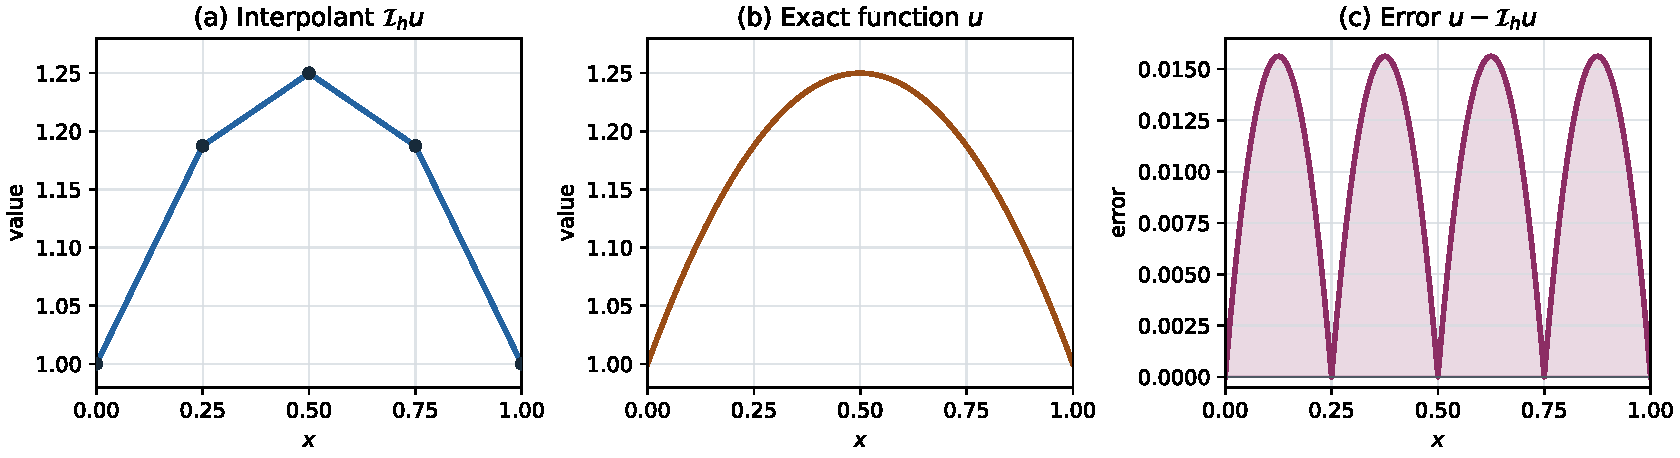
\includegraphics[width=0.96\textwidth]{c7_interpolation_1d.pdf}

  \vspace{0.08cm}
  On every element,
  \[
    u(x)-\mathcal I_eu(x)
    =(x-x_e)(x_{e+1}-x).
  \]
  Since $h=1/4$ on each element, the error reaches the same maximum
  $h^2/4=1/64$ at every element midpoint.
\end{frame}

\begin{frame}{Interpolation on eight linear elements}
  \centering
  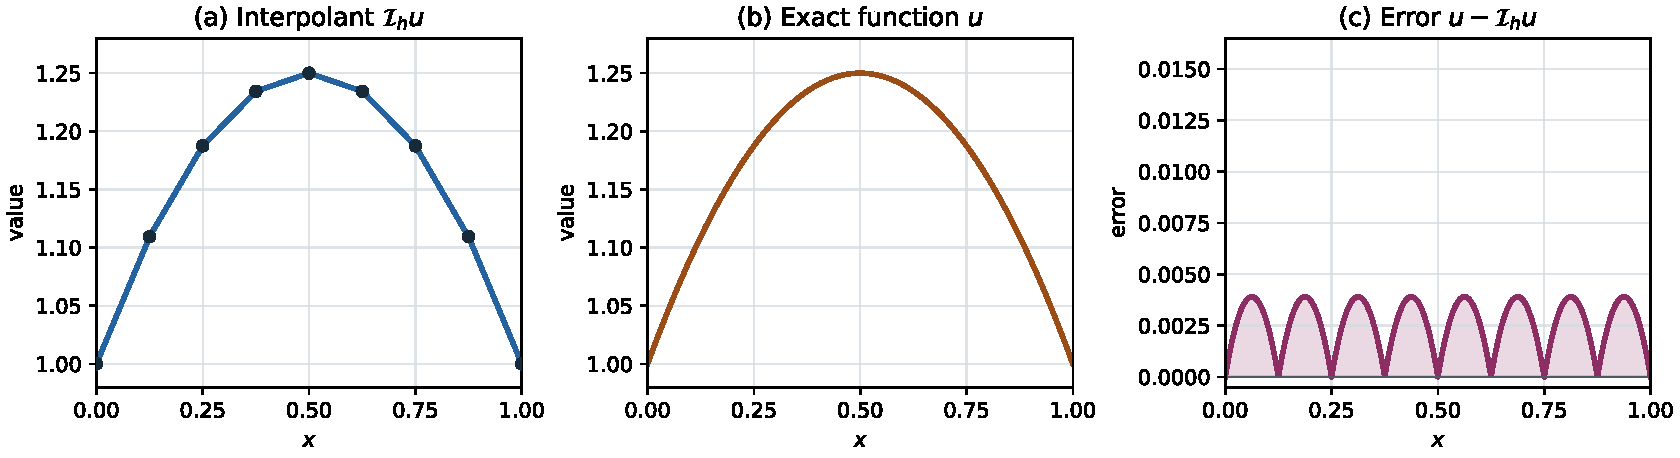
\includegraphics[width=0.96\textwidth]{c7_interpolation_1d_fine.pdf}

  \vspace{0.08cm}
  Dividing every coarse element in two gives nine nodes
  $x_i=(i-1)/8$. The element length decreases from $1/4$ to $1/8$, and the
  maximum error decreases from $1/64$ to $1/256$.
\end{frame}

\begin{frame}{Local interpolation estimates}
Let $\mathcal K_e=(x_e,x_{e+1})$, $h_e=x_{e+1}-x_e$, and
$u\in H^2(\mathcal K_e)$. Then
\[
  \boxed{
  \norm[L^2(\mathcal K_e)]{(u-\mathcal I_eu)'}
  \leq
  h_e\norm[L^2(\mathcal K_e)]{u''}}
\]
and
\[
  \boxed{
  \norm[L^2(\mathcal K_e)]{u-\mathcal I_eu}
  \leq
  h_e^2\norm[L^2(\mathcal K_e)]{u''}.}
\]

The derivative error contains one power of $h_e$. The error in the function
values contains two powers of $h_e$.
\end{frame}

\begin{frame}{Derivative estimate on one element}
Set
\[
  w=u-\mathcal I_eu.
\]
Because $\mathcal I_eu$ is linear, $w''=u''$. Also,
\[
  w(x_e)=w(x_{e+1})=0.
\]
Rolle's theorem gives $x_*\in(x_e,x_{e+1})$ such that $w'(x_*)=0$. Hence
\[
  w'(y)=\int_{x_*}^{y}w''(t)\,\dd t.
\]
Cauchy--Schwarz gives
\[
  |w'(y)|^2
  \leq h_e\norm[L^2(\mathcal K_e)]{w''}^2.
\]
Integrating over an interval of length $h_e$ yields
\[
  \norm[L^2(\mathcal K_e)]{w'}
  \leq h_e\norm[L^2(\mathcal K_e)]{u''}.
\]
\end{frame}

\begin{frame}{$L^2$ estimate on one element}
Use $w(x_e)=0$ and write
\[
  w(y)=\int_{x_e}^{y}w'(t)\,\dd t.
\]
Cauchy--Schwarz and integration over $\mathcal K_e$ give
\[
  \norm[L^2(\mathcal K_e)]{w}
  \leq h_e\norm[L^2(\mathcal K_e)]{w'}.
\]
Combining this relation with the derivative estimate gives
\[
  \norm[L^2(\mathcal K_e)]{u-\mathcal I_eu}
  \leq h_e^2\norm[L^2(\mathcal K_e)]{u''}.
\]

The two powers of $h_e$ arise from two applications of the fundamental
theorem of calculus and the Cauchy--Schwarz inequality.
\end{frame}

\begin{frame}{From local estimates to global estimates}
Because the elements have disjoint interiors,
\[
  \seminorm[H^1(0,L)]{u-\mathcal I_hu}^2
  =\sum_{e=1}^{N}
  \norm[L^2(\mathcal K_e)]{(u-\mathcal I_eu)'}^2,
\]
and
\[
  \norm[L^2(0,L)]{u-\mathcal I_hu}^2
  =\sum_{e=1}^{N}
  \norm[L^2(\mathcal K_e)]{u-\mathcal I_eu}^2.
\]
Applying the local bounds gives
\[
  \seminorm[H^1(0,L)]{u-\mathcal I_hu}^2
  \leq\sum_{e=1}^{N}h_e^2
  \norm[L^2(\mathcal K_e)]{u''}^2,
\]
\[
  \norm[L^2(0,L)]{u-\mathcal I_hu}^2
  \leq\sum_{e=1}^{N}h_e^4
  \norm[L^2(\mathcal K_e)]{u''}^2.
\]
\end{frame}

\begin{frame}{What to retain from today}
\begin{itemize}
  \item Continuity and coercivity provide a stable continuous and discrete
  problem.
  \item Galerkin orthogonality compares the finite element error with every
  function in the discrete space.
  \item C\'ea's lemma bounds the error by the best approximation available in
  that space.
  \item For symmetric problems, the finite element solution is the best
  approximation in the energy norm.
  \item The nodal interpolant gives a specific finite element function whose
  error can be bounded in terms of $h$ and derivatives of $u$.
\end{itemize}

\vspace{0.2cm}
The next part of Chapter 7 extends the interpolation estimate to
multidimensional elements and then combines it with C\'ea's lemma.
\end{frame}

\end{document}
